\begin{enumerate}
 \item Le vecteur $\overrightarrow{e}_t$ étant défini relativement à un repère orthonormé dont les fonctions coordonnées sont notées $x$ et $y$. L'énoncé n'est pas très explicite mais définit $\Gamma$ comme le support de la courbe paramétrée ($\theta \in \R$)
\begin{displaymath}
 f(\theta) = O + (1+\cos t)\overrightarrow{e}_\theta
\end{displaymath}
On peut restreindre l'espace de définition à $]-\pi , +\pi [$ car la fonction est clairement $2\pi$ périodique. L'origine du repère est le point associé aux valeurs $-\pi$ et $\pi$ du paramètre. On convient donc de l'enlever de $\Gamma$.\newline
 On peut exprimer $x(f(\theta))$ et $y(f(\theta))$ en fonction de $\tan\frac{\theta}{2}$ :
\begin{align*}
 x(f(\theta)) = 2\dfrac{1-\tan\frac{\theta}{2}^2}{(1+\tan\frac{\theta}{2}^2)^2} & & 
 y(f(\theta)) = \dfrac{4\tan\frac{\theta}{2}}{(1+\tan\frac{\theta}{2}^2)^2}
\end{align*}
On en déduit que $g\circ \varphi = f$ avec
\begin{displaymath}
 g(t) = 0 + 2\dfrac{1-t^2}{(1+t^2)^2}\overrightarrow i + \dfrac{4t}{(1+t^2)^2}\overrightarrow j
\end{displaymath}
Les courbes paramétrées $f$ et $g$ ont donc le même support $\Gamma$, la fonction $\varphi$ réalisant un changement de paramètre admissible entre les deux\index{changement de paramètre admissible}.
\item Notons respectivement $u$ et $v$ les fonctions $x\circ g$ et $y\circ g$ :
\begin{align*}
 u(t) = 2\dfrac{1-t^2}{(1+t^2)^2} & & v(t) = \dfrac{4t}{(1+t^2)^2}
\end{align*}
Pour préciser une direction de tangente, on calcule $u^\prime$ et $v^\prime$ en s'attachant à factoriser. On obtient
\begin{displaymath}
 \overrightarrow{g^\prime}(t) = u^\prime(t)\overrightarrow i +v^\prime(t)\overrightarrow j
= -\dfrac{4}{(1+t^2)^3}\left( (-t^3+3t)\overrightarrow i +(3t^2-1)\overrightarrow j\right)  
\end{displaymath}
On en déduit que la direction de la tangente au point de paramètre $\sqrt{3}$ est $\overrightarrow j$ car le $-t^3+3t$ (coefficient de $\overrightarrow i$) s'annule.

\item D'après le calcul précédent, l'équation de la tangente (notée $\mathcal T_\tau$) en $M=g(\tau)$ est :
\begin{equation*}
 \begin{vmatrix}
  x - \dfrac{2(1-\tau^2)}{(1+\tau^2)^2} & -\tau^3 + 3\tau \\
 y - \dfrac{4\tau}{(1+\tau^2)^2}& -1+3\tau^2
 \end{vmatrix}
=0
\end{equation*}
ce qui s'écrit encore
\begin{equation*}
 (3\tau^2-1)x + (\tau^3-3\tau)y + \dfrac{1}{(1+\tau^2)^2} \left( 
 2(1-\tau^2)(1-3\tau^2) -4\tau(\tau^3-3\tau^2)
\right) =0
\end{equation*}
En fait, la dernière parenthèse se réduit à
\begin{displaymath}
 2(1+\tau^2)^2
\end{displaymath}
ce qui conduit à l'équation de la tangente annoncée :
\begin{equation*}
 (\tau^3-3\tau)y+(3\tau^2-1)x+2=0
\end{equation*}

\item Formons l'équation d'inconnue $t$ caractérisant que $g(t)\in\Gamma$. Après multiplication par $(1+t^2)^2\neq0$ elle s'écrit :
\begin{equation*}
 (\tau^3-3\tau)4t + 2(3\tau^2-1)(1-t^2)+ 2(1+t^2)^2 = 0
\end{equation*}
Cette équation est de degré $4$ et l'énoncé 
\footnote{voir à la fin du coorigé} nous indique qu'elle s'écrit
\begin{equation*}
 T^2\left( T^2+4\tau T +3(\tau^2 +1) \right)
\end{equation*}
lorsque $t=\tau+T$. Cela montre que $\tau$ est racine (double) de cette équation et que $\mathcal T_t$ recoupe $\Gamma$ aux points $g(t)$ pour $t=\tau + u$ avec $u$ racine de
\begin{equation*}
 T^2 +4\tau T +3(\tau^2+1)
\end{equation*}
d'inconnue $T$. Le discriminant de cette équation est
\begin{displaymath}
 16\tau^2 -12(\tau^2 +1) = 4(\tau^2 -3)
\end{displaymath}
Ceci montre que $\mathcal T_t$ recoupe $\Gamma$ en deux points si et seulement si $\tau^2 > 3$.
Lorsque cette condition est réalisée, l'équation admet deux solutions $u_1$ et $u_2$ vérifiant :
\begin{equation*}
\left\lbrace 
 \begin{aligned}
  u_1 + u_2 &= -4 \tau \\
 u_1u_2 &= 3(\tau^2 +1)
 \end{aligned}
\right. 
\end{equation*}
(relation entre coefficients et racines dans une équation du second degré) \index{relation entre coefficient et racines}\newline
La tangente $\mathcal T_t$ recoupe $\Gamma$ en deux points $g(t_1)$ et $g(t_2)$ avec $t_1=\tau +u_1$ et $t_2=\tau +u_2$. On en déduit :
\begin{align*}
 t_1t_2 &= \tau^2 + \tau(u_1+u_2) = u_1u_2 = 3 \\
 t_1 + t_2 &= 2\tau -4\tau = -2 \tau
\end{align*}

\item \begin{enumerate}
 \item En utilisant les relations précédentes, on obtient après calculs :
\begin{equation*}
 \begin{vmatrix}
    t_1^3-3t_1 & 3t_1^2-1 \\
    t_2^3-3t_2 & 3t_2^2-1
 \end{vmatrix}
 = (60-4\tau^2)(t_1 -t_2)
\end{equation*}

\item Le système d'équation régissant l'intersection des tangentes $\mathcal T_{t_1}$ et $\mathcal T_{t_2}$ est :
\begin{equation*}
 \left\lbrace 
\begin{aligned}
 (3t_1 -1)x + (t_1^3 -3t_1)y &= -2 \\
(3t_2 -1)x + (t_2^3 -3t_2)y &= -2
\end{aligned}
\right. 
\end{equation*}
Le déterminant a été calculé en a. Les formules de Cramer\index{formules de Cramer} conduisent à :
\begin{align*}
 x &= \dfrac
{
\begin{vmatrix}
 -2 & t_1^3 -3t_1\\
 -2 & t_2^3 -3t_2
\end{vmatrix}
}
{(60-4\tau^2)(t_1-t_2)}
 = \dfrac{2\tau^2 - 3}{\tau^2 - 15}\\
y &= \dfrac
{
\begin{vmatrix}
 3t_1^2 -1 & -2 \\
 3t_2^2 -1 & -2
\end{vmatrix}
}
{(60-4\tau^2)(t_1-t_2)}
= \dfrac{3\tau}{\tau^2-15}
\end{align*}
\end{enumerate}

\item Lorsque la tangente en $M=g(\tau)$ recoupe $\Gamma$ en deux autres points, les tangentes en ces points se coupent en $N_\tau$ dont les coordonnées sont :
\begin{align*}
  x_\tau = \dfrac{2\tau^2 - 3}{\tau^2 - 15}  & & y_\tau = \dfrac{3\tau}{\tau^2-15}
\end{align*}
La première relation permet d'exprimer $\tau^2$ puis $\tau^2 -15$ en fonction de $x_\tau$ :
\begin{align*}
 \tau^2 = \dfrac{-3+15x}{x_\tau-2} & & \tau^2 -15 = \dfrac{27}{x_\tau-2}
\end{align*}
La deuxième relation permet alors d'exprimer $\tau$ en fonction de $x_\tau$ et de $y_\tau$ :
\begin{displaymath}
 \tau = \dfrac{9y_\tau}{x_\tau-2}
\end{displaymath}
En remplaçant dans la relation exprimant $\tau^2$ en fonction de $x_\tau$, on obtient l'équation d'une courbe qui contient tous les points $N_\tau$.
\begin{equation*}
 \left( \dfrac{9y_\tau}{x_\tau-2}\right) ^2 = \dfrac{3(5x_\tau-1)}{x_\tau-2} \Leftrightarrow
5x_\tau^2 -27y_\tau^2 - 11x_\tau+2 =0
\end{equation*}

\begin{figure}[h]
 \centering
 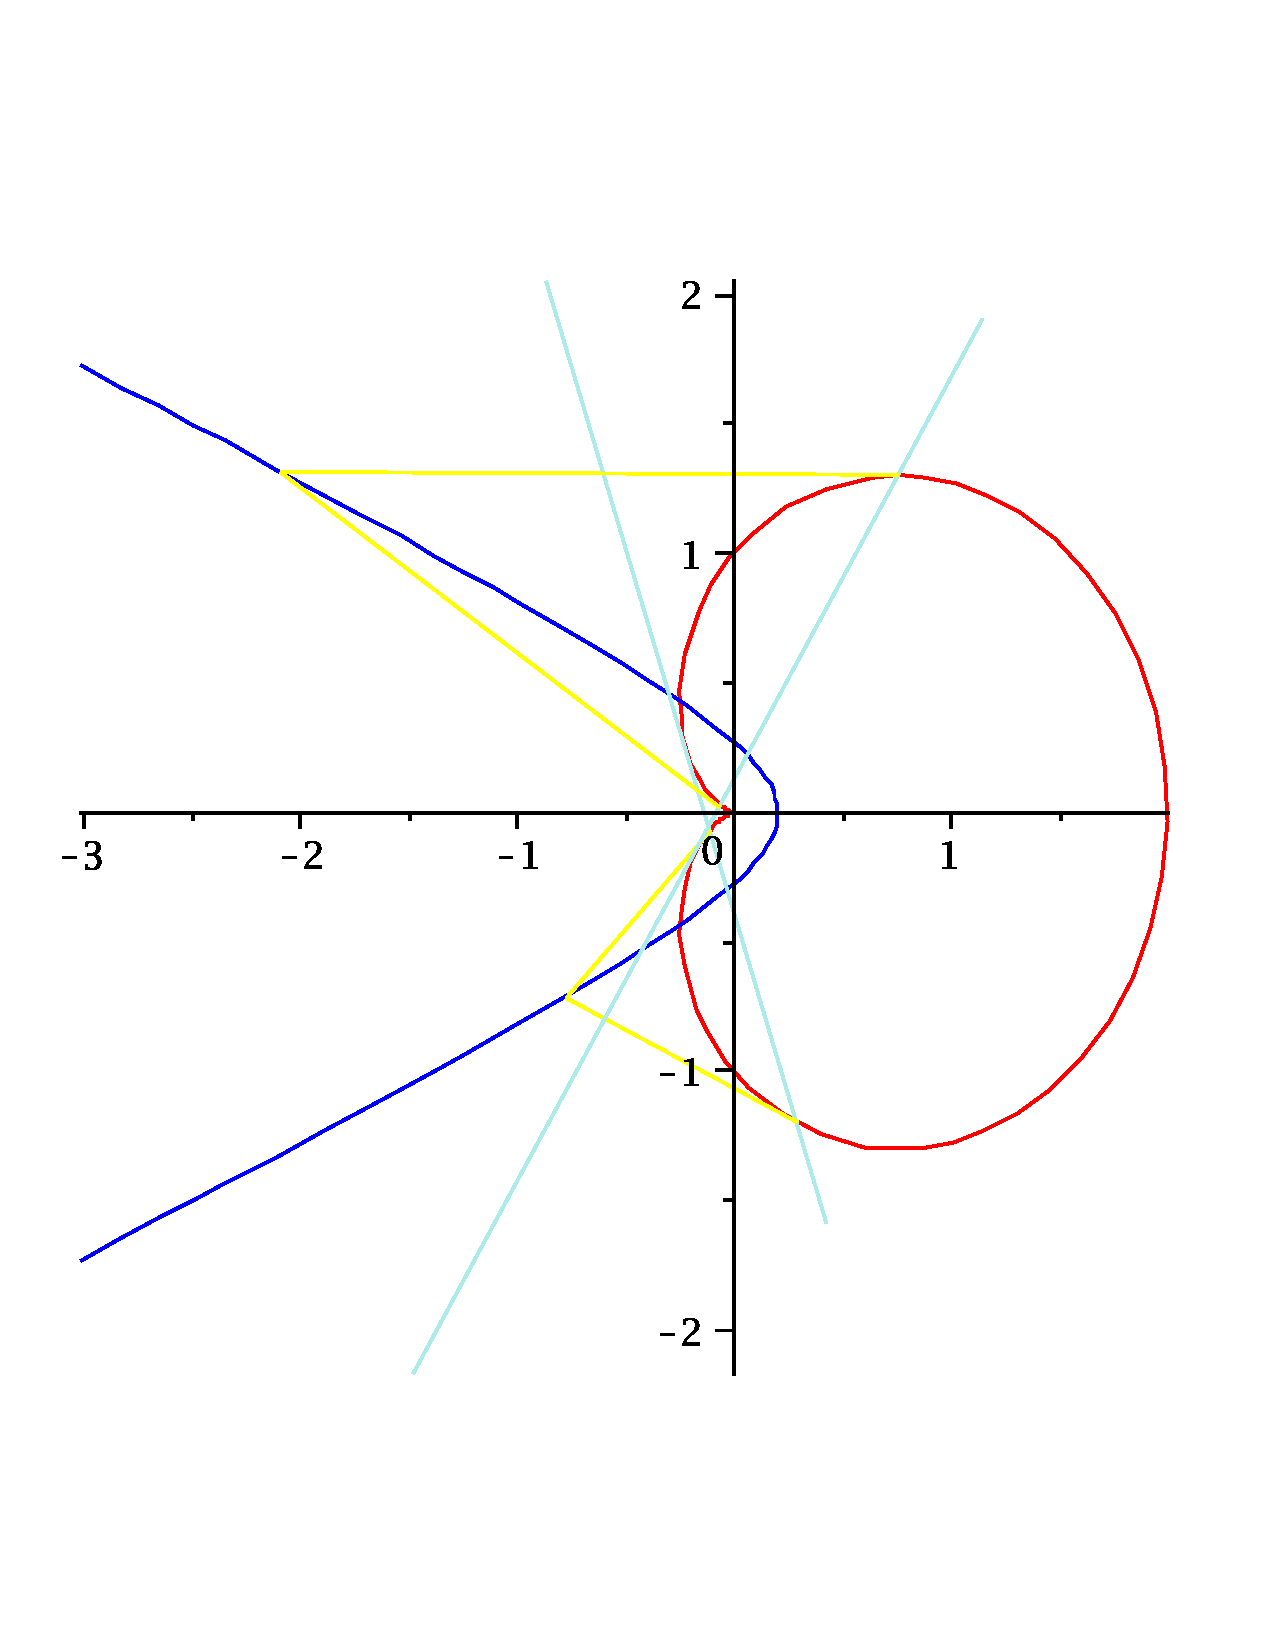
\includegraphics[width=8cm]{Ccardioid_1.pdf}
 % Ccardioid_1.pdf: 612x792 pixel, 72dpi, 21.59x27.94 cm, bb=0 0 612 792
\caption{Question 7.}
\end{figure}
\item Pour mettre l'équation précédente sous la forme d'une équation réduite de conique, on considère les termes en $x$ et $x^2$ comme le début d'un carré comme dans la méthode de factorisation canonique. On obtient une hyperbole d'équation réduite
\begin{equation*}
 \dfrac{\left( x - \dfrac{11}{10}\right)^2 }{\left( \dfrac{9}{10}\right)^2 }
- \dfrac{y^2}{\left( \dfrac{\sqrt{3}}{2\sqrt{5}}\right)^2}
= 1
\end{equation*}
d'axe focal $Ox$, de centre le point de coordonnées $(\frac{11}{10},0)$
\end{enumerate}

\subsubsection*{Annexe}
Les lignes de code suivantes permettent de réaliser avec Maple la substitution utilisée en question 4.
\begin{verbatim*}
A:=(3*tau^2-1)*(1-t^2)+(tau^3-3*tau)*2*t+(1+t^2)^2;
expand(subs(t=T+tau,A));
\end{verbatim*}
